\begin{figure}[t]
    \centering
    \begin{tikzpicture}
    \pgfplotsset{footnotesize,samples=10}
    \begin{groupplot}[group style = {group size = 3 by 1, horizontal sep = 30pt}, width = 5.0cm, height = 4.5cm]


\nextgroupplot[title = {CraisglistBargain},
legend style = { column sep = 10pt, legend columns = -1, legend to name = grouplegend2}, 
    ylabel={Relative Success Rate \%}, 
            xlabel={Turn of Conversation},
    xmin=0, xmax=8,
    ymin=-5, ymax=25,
    xtick={0,1,2,3,4,5,6,7,8},
    ytick={-5,0,5,15,25}, grid=both,
    grid style={dashed, gray!50},]

\addplot[
    color=blue,
    mark=square,
    ]
    coordinates {
    (0,0.00)(1,0.00)(2,4.25)(3,14.37)(4,14.36)(5,9.58)(6,7.97)(7,7.44)(8,7.44)
    };

\addplot[
    color=orange,
    mark=triangle,
    ]
    coordinates {
    (0,0.00)(1,0.53)(2,-0.53)(3,-1.06)(4,3.19)(5,5.85)(6,11.17)(7,15.96)(8,17.02)
    };

\addplot[
    color=green, mark=diamond,
    ]
    coordinates {
    (0,0.00)(1,0.00)(2,3.72)(3,6.39)(4,10.64)(5,15.96)(6,17.02)(7,18.61)(8,18.61)
    };

\addplot[
    color=purple, mark=x,
    ]
    coordinates {
    (0,0.00)(1,0.00)(2,0.53)(3,1.60)(4,-0.53)(5,-0.53)(6,-1.07)(7,-0.53)(8,-0.53)
    };

\addplot[
    color=red,
    mark=o,
    ]
    coordinates {
    (0,0.00)(1,0.00)(2,2.13)(3,1.60)(4,18.09)(5,20.22)(6,21.27)(7,21.81)(8,22.87)
    };

    
    \addlegendentry{AnE}
    \addlegendentry{Proactive}
    \addlegendentry{ProCoT}
    \addlegendentry{ICL-AIF}
    \addlegendentry{PPDPP}
    
\nextgroupplot[ title = {ESConv},
    xlabel={Turn of Conversation},
    xmin=0, xmax=8,
    ymin=-5, ymax=12,
    xtick={0,1,2,3,4,5,6,7,8},
    ytick={-5,0,5,10}, grid=both,
    grid style={dashed, gray!50},]


\addplot[
    color=blue,
    mark=square,
    ]
    coordinates {
    (0,0.00)(1,2.70)(2,5.38)(3,5.39)(4,5.39)(5,6.16)(6,3.08)(7,0.77)(8,3.08)
    };

\addplot[
    color=orange,
    mark=triangle,
    ]
    coordinates {
    (0,0.00)(1,5.39)(2,0.38)(3,1.16)(4,-0.38)(5,-1.92)(6,-1.15)(7,-1.92)(8,1.54)
    };

\addplot[
    color=green, mark=diamond,
    ]
    coordinates {
    (0,0.00)(1,0.77)(2,7.30)(3,7.31)(4,1.20)(5,0.72)(6,1.77)(7,2.69)(8,0.77)
    };

\addplot[
    color=purple, mark=x,
    ]
    coordinates {
    %(0,0.00)(1,1.54)(2,8.84)(3,5.77)(4,0.39)(5,1.93)(6,-0.38)(7,-0.39)(8,5.00)
    (0,0.00)(1,1.54)(2,8.84)(3,5.77)(4,4.39)(5,5.93)(6,3.38)(7,4.39)(8,5.00)
    };

\addplot[
    color=red,
    mark=o,
    ]
    coordinates {
    (0,0.00)(1,4.62)(2,5.77)(3,9.62)(4,6.38)(5,7.70)(6,6.38)(7,6.92)(8,6.54)
    };
    
\nextgroupplot[title = {CIMA},xlabel={Turn of Conversation},
    xmin=0, xmax=8,
    ymin=-20, ymax=20,
    xtick={0,1,2,3,4,5,6,7,8},
    ytick={-20,-10,0,10,20}, grid=both,
    grid style={dashed, gray!50},]

\addplot[
    color=blue,
    mark=square,
    ]
    coordinates {
    (0,0.00)(1,16.82)(2,2.66)(3,-1.77)(4,-3.54)(5,-3.54)(6,-3.54)(7,-3.54)(8,-3.54)
    };

\addplot[
    color=orange,
    mark=triangle,
    ]
    coordinates {
    (0,0.00)(1,-4.42)(2,-17.70)(3,-13.28)(4,-11.50)(5,-11.50)(6,-10.62)(7,-11.50)(8,-12.39)
    };

\addplot[
    color=green, mark=diamond,
    ]
    coordinates {
    (0,0.00)(1,2.66)(2,-9.74)(3,-13.27)(4,-15.04)(5,-15.04)(6,-15.93)(7,-15.93)(8,-16.82)
    };

\addplot[
    color=purple, mark=x,
    ]
    coordinates {
    (0,0.00)(1,7.08)(2,-5.31)(3,-6.20)(4,-6.20)(5,-5.31)(6,-6.20)(7,-7.08)(8,-7.97)
    };

\addplot[
    color=red,
    mark=o,
    ]
    coordinates {
    (0,0.00)(1,16.82)(2,-7.08)(3,9.74)(4,16.81)(5,17.70)(6,16.81)(7,15.93)(8,15.04)
    };

    
    \end{groupplot}
    \node at ($(group c2r1) + (0,-2.7cm)$) {\ref{grouplegend2}}; 
\end{tikzpicture}
    \vspace{-0.4cm}
    \caption{Comparisons of relative success rate against Standard at different conversation turns.}
    \vspace{-0.5cm}
    \label{fig:exp-turn}
\end{figure}


\begin{wrapfigure}{R}{5.5cm}
    \centering
    \vspace{-1.8cm}
    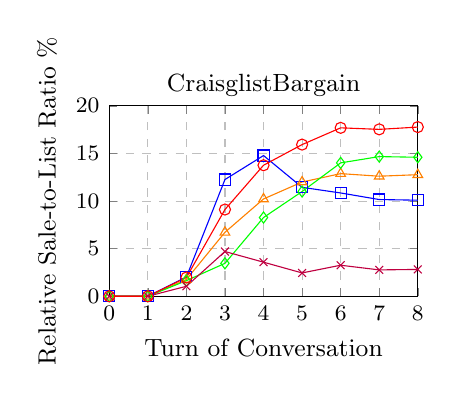
\begin{tikzpicture}
    \pgfplotsset{footnotesize,samples=10}
    \begin{axis}[ title = {CraisglistBargain},
    legend style = { column sep = 10pt, legend to name = legend, at={(0,0)}}, 
    xlabel={Turn of Conversation},
    ylabel={Relative Sale-to-List Ratio \%},
    xmin=0, xmax=8,
    ymin=-0, ymax=20,
    xtick={0,1,2,3,4,5,6,7,8},
    ytick={0,5,10,15,20}, 
    grid=both,
    grid style={dashed, gray!50},width = 5.5cm, height = 4cm]

\addplot[
    color=blue,
    mark=square,
    ]
    coordinates {
    (0,0.00)(1,0.00)(2,2.02)(3,12.26)(4,14.78)(5,11.44)(6,10.85)(7,10.16)(8,10.09)
    };

\addplot[
    color=orange,
    mark=triangle,
    ]
    coordinates {
    (0,0.00)(1,0.00)(2,1.76)(3,6.72)(4,10.22)(5,12.00)(6,12.88)(7,12.61)(8,12.77)
    };

\addplot[
    color=green, mark=diamond,
    ]
    coordinates {
    (0,0.00)(1,0.00)(2,1.64)(3,3.46)(4,8.27)(5,11.00)(6,14.01)(7,14.67)(8,14.60)
    };

\addplot[
    color=purple, mark=x,
    ]
    coordinates {
    (0,0.00)(1,0.00)(2,1.05)(3,4.70)(4,3.58)(5,2.45)(6,3.26)(7,2.77)(8,2.82)
    };

\addplot[
    color=red,
    mark=o,
    ]
    coordinates {
    (0,0.00)(1,0.00)(2,1.97)(3,9.11)(4,13.76)(5,15.93)(6,17.69)(7,17.53)(8,17.77)
    };
    
    \addlegendentry{AnE}
    \addlegendentry{Proactive}
    \addlegendentry{ProCoT}
    \addlegendentry{ICL-AIF}
    \addlegendentry{PPDPP}
    
    \end{axis}
    %\node at ($(group c2r1) + (-1cm,-0.5cm)$) {\ref{legend}}; 
\end{tikzpicture}
    \vspace{-0.3cm}
    \caption{Comparisons of relative Sale-to-List Ratio against Standard at different turns (same legends as Figure \ref{fig:exp-turn}).}
    \label{fig:exp-turn-slr}
    \vspace{-0.4cm}
\end{wrapfigure}